\pdfinfoomitdate=1
\pdfsuppressptexinfo=15
\pdftrailerid{}
\documentclass[journal]{IEEEtran}

\usepackage[T1]{fontenc}
\usepackage{mathptmx}
\usepackage{textcomp}
\usepackage{amsmath,amssymb}
\usepackage{graphicx}
\usepackage{tikz}
\usetikzlibrary{arrows.meta,positioning,fit,calc}
\usepackage{booktabs}
\usepackage{tabularx}
\usepackage{array}
\usepackage{cite}
\usepackage{url}
\usepackage{balance}
\usepackage[hidelinks,
  pdftitle={Bullet Farm: A Software-Change Transaction Processor for Heterogeneous Agents},
  pdfauthor={Bullet Farm Maintainers},
  pdfsubject={Architecture and component-assurance preprint},
  pdfkeywords={software-change transactions, coding agents, Git isolation, evidence binding, authority fencing}]{hyperref}

% Generated from evidence.json by scripts/paper-build.sh. Do not edit.
\newcommand{\EvidenceSnapshotId}{20260825-stage1-r3}
\newcommand{\EvidenceSnapshotDate}{2026-08-25}
\newcommand{\EvidenceStage}{architecture-component-assurance}
\newcommand{\EvidenceHubCommit}{3039878371b6}
\newcommand{\EvidenceKernelCommit}{ca380bc4ffd4}
\newcommand{\EvidenceGitCommit}{fb715b25c3b2}
\newcommand{\EvidencePortalCommit}{95108e37d643}
\newcommand{\EvidenceDoctorOutcome}{BLOCKED}
\newcommand{\EvidenceReleaseOutcome}{BLOCKED}
\newcommand{\EvidenceReleaseEvaluated}{26}
\newcommand{\EvidenceReleaseBlocked}{26}
\newcommand{\EvidenceFastOutcome}{PASS}
\newcommand{\EvidenceDemoOutcome}{PASS}
\newcommand{\EvidenceFormalOutcome}{PASS}
\newcommand{\EvidenceFormalModels}{2}
\newcommand{\EvidenceAuditScore}{58}
\newcommand{\EvidenceAuditRaw}{58}
\newcommand{\EvidenceAuditCaps}{10}
\newcommand{\EvidenceAuditHard}{29}
\newcommand{\EvidenceAuditSoft}{15}
\newcommand{\EvidenceTransactionOutcome}{ABSENT}

% Shared vector figure used by the IEEE paper and executive brief.
\newcommand{\BulletArchitectureFigure}[1]{%
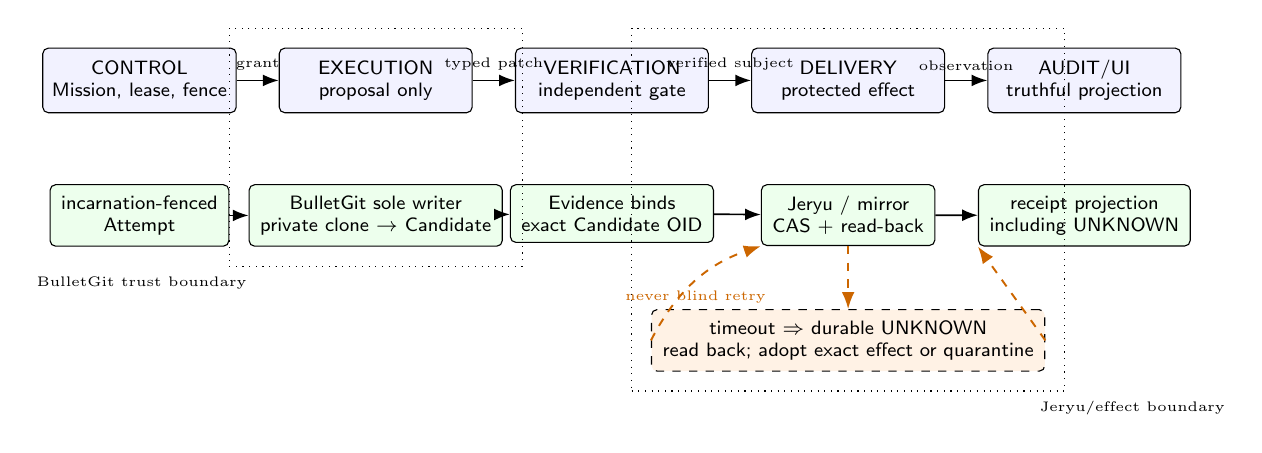
\begin{tikzpicture}[
  x=1cm,y=1cm,>=Latex,
  plane/.style={draw,rounded corners=2pt,minimum width=2.45cm,minimum height=.82cm,align=center,font=\sffamily\scriptsize,fill=blue!5},
  subject/.style={draw,rounded corners=2pt,align=center,font=\sffamily\scriptsize,fill=green!7,inner sep=4pt},
  warning/.style={draw,dashed,rounded corners=2pt,align=center,font=\sffamily\scriptsize,fill=orange!10,inner sep=4pt},
  flow/.style={->,line width=.6pt},
  reconcile/.style={->,dashed,line width=.7pt,color=orange!80!black}
]
\node[plane] (control) at (0,0) {CONTROL\\Mission, lease, fence};
\node[plane] (execution) at (3.0,0) {EXECUTION\\proposal only};
\node[plane] (verification) at (6.0,0) {VERIFICATION\\independent gate};
\node[plane] (delivery) at (9.0,0) {DELIVERY\\protected effect};
\node[plane] (audit) at (12.0,0) {AUDIT/UI\\truthful projection};

\node[subject,below=.9cm of control] (attempt) {incarnation-fenced\\Attempt};
\node[subject,below=.9cm of execution] (candidate) {BulletGit sole writer\\private clone $\rightarrow$ Candidate};
\node[subject,below=.9cm of verification] (evidence) {Evidence binds\\exact Candidate OID};
\node[subject,below=.9cm of delivery] (effect) {Jeryu / mirror\\CAS + read-back};
\node[subject,below=.9cm of audit] (projection) {receipt projection\\including UNKNOWN};

\draw[flow] (control) -- node[above,font=\tiny]{grant} (execution);
\draw[flow] (execution) -- node[above,font=\tiny]{typed patch} (verification);
\draw[flow] (verification) -- node[above,font=\tiny]{verified subject} (delivery);
\draw[flow] (delivery) -- node[above,font=\tiny]{observation} (audit);
\draw[flow] (attempt) -- (candidate);
\draw[flow] (candidate) -- (evidence);
\draw[flow] (evidence) -- (effect);
\draw[flow] (effect) -- (projection);

\node[warning,below=.8cm of effect] (unknown) {timeout $\Rightarrow$ durable UNKNOWN\\read back; adopt exact effect or quarantine};
\draw[reconcile] (effect) -- (unknown);
\draw[reconcile] (unknown.west) to[bend left=22] node[below,font=\tiny]{never blind retry} (effect.south west);
\draw[reconcile] (unknown.east) -- (projection.south west);

\node[draw,dotted,fit=(execution)(candidate),inner sep=7pt,label={[font=\tiny]below left:BulletGit trust boundary}] {};
\node[draw,dotted,fit=(delivery)(effect)(unknown),inner sep=7pt,label={[font=\tiny]below right:Jeryu/effect boundary}] {};
\end{tikzpicture}%
}


\hyphenation{Bullet-Git Gas-Town Gas-City Omni-gent Deep-Seek work-tree}
\newcommand{\Designed}{\textsf{Designed}}
\newcommand{\ComponentProved}{\textsf{Component-proved}}
\newcommand{\TransactionProved}{\textsf{Transaction-proved}}
\newcommand{\LiveReleaseProved}{\textsf{Live/release-proved}}
\newcommand{\Doc}{\textsf{Documented}}
\newcommand{\Partial}{\textsf{Partial/configuration-dependent}}
\newcommand{\NotDoc}{\textsf{Not documented}}
\newcommand{\Unknown}{\textsf{Unknown}}
\newcommand{\NA}{\textsf{N/A}}
\newcommand{\code}[1]{\texttt{\detokenize{#1}}}

\begin{document}

\title{Bullet Farm: A Software-Change Transaction Processor for Heterogeneous Agents}

\author{Bullet~Farm~Maintainers%
\thanks{Bullet Farm split-family maintainers. This architecture and component-assurance preprint is not a release receipt or a benchmark result.}%
}

\markboth{Bullet Farm Technical Preprint, August 2026}{Bullet Farm Maintainers: A Software-Change Transaction Processor}
\maketitle

\begin{abstract}
Coding agents are now capable enough that their limiting failure is often not
reasoning but the authority around it: two sessions edit one checkout, a
review approves bytes that no longer exist, a timed-out push is retried after
the server applied it, and a dashboard paints silence green. Bullet Farm is a
software-change transaction processor \emph{around} heterogeneous agents. Its
binding chain---incarnation-fenced authority, one repository writer, private
Attempt clones, exact-OID Candidates, independently bound Evidence, durable
effect intent, read-back and adoption after ambiguity, and truthful
\code{UNKNOWN} projection across five trust planes---is designed to remove
seven concrete failure classes and to leave every integrated change with
exact, replayable evidence of who observed which bytes under which gate. The
upside, if it works, is verified autonomous software change whose cost,
refusal rate, and unresolved unknowns are measured rather than inferred; none
of it is claimed as measured here. Evidence is labelled \Designed,
\ComponentProved, \TransactionProved, or \LiveReleaseProved. At snapshot
\EvidenceSnapshotId{} nothing exceeds \ComponentProved: two bounded TLA+
safety models and the component lanes pass, while the connected
\code{TRANSACTION_PROOF}, every live provider/forge receipt, and the release
are absent, and the release inventory reports \EvidenceReleaseBlocked{}
blocked of \EvidenceReleaseEvaluated{} evaluated gates. The biggest concerns
are ranked with mitigations and retiring evidence: an unassembled connected
product, absent live evidence, dependence on operator custody acts, a
single-host Linux-only threat model, holdout-dependent verifier independence,
a security score below its own floor, bounds the design cannot eliminate, and
system size and cost. Comparison with a dated public corpus (Gas Town v1.2.1,
Gas City v1.4.1, DeepSeek Harness dsh-v0.1.1-rc.2, Omnigent v0.10.0) makes no
performance or superiority claim; a Stage-2 matched benchmark waits for the
connected transaction proof.
\end{abstract}

\begin{IEEEkeywords}
coding agents, transaction processing, Git isolation, evidence binding,
authority fencing, effect reconciliation, merge safety.
\end{IEEEkeywords}

\section{Research Contract}
\label{sec:contract}

Agent systems are capable enough that their limiting failure is often not
model reasoning but the authority surrounding it. Classical
transaction-processing work treats identity, concurrency, logging, recovery,
and idempotence as one problem~\cite{gray1981,gray1993,helland2012};
coding-agent stacks distribute those obligations among an editor, Git, CI, a
provider process, and a forge without an end-to-end subject binding.

Bullet Farm's thesis is narrower than ``better agents'': it is a
software-change transaction processor \emph{around} heterogeneous agents,
where a model may reason, search, and propose but cannot mint its own write,
verification, or integration authority~\cite{bulletOverview}. The research
questions are:

\begin{description}
\item[RQ1:] Which identities and exact subjects must be bound so that a
concurrent agent run can be recovered without inferring completion?
\item[RQ2:] Which bindings are implemented and component-proved in the current
family, and which remain design or connected-product gaps?
\item[RQ3:] Do the reviewed pinned public contracts of adjacent systems
document the same end-to-end bindings, after separating operational capability
from authority and integrity?
\item[RQ4:] What observations would falsify the design, and what matched
experiment would be required before a comparative performance claim?
\end{description}

\subsection{Inclusion and Source Discipline}

Deep studies were included when a system exposed a public architecture plus a
release or commit suitable for reproducible inspection: Gas Town v1.2.1, Gas
City v1.4.1, DeepSeek Harness dsh-v0.1.1-rc.2, and Omnigent
v0.10.0~\cite{gastownV121,gascityV141,dshV011,omnigentV010}. Issue reports
were included only when they described a concrete authority, Git, evidence, or
recovery failure mappable to a named invariant. The landscape appendix uses
release/commit pins for open-source systems and official-document observation
dates for proprietary ones; these are public-contract observations, not
reverse engineering, and Codex statements rely only on official OpenAI
documentation~\cite{openaiCodexCli,openaiCodexCloud}.

Every comparison cell uses exactly one of five terms: \Doc{} (a pinned primary
source describes the property), \Partial{} (it depends on configuration or
covers part of the row), \NotDoc{} (the reviewed sources do not describe it,
which does not assert the implementation lacks it), \Unknown{} (the public
material was insufficient to classify), and \NA{} (outside the product's
stated role). Absence of documentation is never a categorical ``No.''

\subsection{Evidence Vocabulary and Claim Limit}

Table~\ref{tab:maturity} is the paper's claim lattice; the terms avoid the
ambiguous word ``complete'' and are generated into both documents from
\code{evidence.json}, schema
\code{bullet.paper-evidence.v1}~\cite{paperEvidence}.

\begin{table}[!t]
\caption{Maturity labels used throughout this paper.}
\label{tab:maturity}
\centering
\scriptsize
\begin{tabularx}{\columnwidth}{@{}p{.28\columnwidth}X@{}}
\toprule
Label & Admitted meaning \\
\midrule
\Designed & Reviewed contract or invariant; no executable receipt required. \\
\ComponentProved & Exact committed component and mapped local receipt; no cross-process transaction inference. \\
\TransactionProved & One exact connected offline five-plane transaction with independent subject-bound receipts. \\
\LiveReleaseProved & Admitted live provider/forge transaction, or signed release/install/recovery proof from the same subjects. \\
\bottomrule
\end{tabularx}
\end{table}

The snapshot records doctor \EvidenceDoctorOutcome, fast lane
\EvidenceFastOutcome, demo \EvidenceDemoOutcome, and \EvidenceFormalOutcome{}
for \EvidenceFormalModels{} bounded formal models. The release result is
written as ``\EvidenceReleaseBlocked{} blocked of \EvidenceReleaseEvaluated{}
evaluated gates,'' never as a bare fraction mistakable for success.
\code{UNKNOWN}, timeout, skipped, unsupported, zero tests, a model assertion,
HTTP 2xx, or process exit zero is not verified engineering
truth~\cite{bulletRelease}, and no result from an active dirty tree enters the
committed evidence manifest.

\subsection{Value and Risk at a Glance}
\label{sec:glance}

Table~\ref{tab:glance} is the two-minute reading of this paper in the
vocabulary of Table~\ref{tab:maturity}; its numbers come from
\code{evidence.json} or Table~\ref{tab:commands}, and
Section~\ref{sec:concerns} expands the ranked concerns.

\begin{table}[!t]
\caption{Value and risk at a glance, snapshot \EvidenceSnapshotId.}
\label{tab:glance}
\centering
\scriptsize
\begin{tabularx}{\columnwidth}{@{}p{.17\columnwidth}X@{}}
\toprule
Question & Answer at this snapshot \\
\midrule
What it is & A transaction processor around coding agents: providers propose; a fenced kernel, one repository writer, an independent verifier, and an effect broker decide what is written, proved, and integrated. \\
Upside if it works & Removes the seven failure classes of Table~\ref{tab:failurebindings}; every integrated change carries exact-subject Evidence naming who observed which bytes under which admitted gate; models and vendors can be swapped without granting any of them repository or merge authority; cost, refusal rate, and unresolved unknowns become measurable, with accepted, surviving change per human intervention and per dollar as the Stage-2 dependent variable, not a claim here; bounded multi-agent evolution is \Designed{} and post-V1. \\
Proven today & \ComponentProved{} only: fast lane \EvidenceFastOutcome, demo \EvidenceDemoOutcome, \EvidenceFormalModels{} bounded safety models \EvidenceFormalOutcome, doctor \EvidenceDoctorOutcome{} by design. \code{TRANSACTION_PROOF} \EvidenceTransactionOutcome; live and release proof absent; \EvidenceReleaseBlocked{} blocked of \EvidenceReleaseEvaluated{} release gates; audit \EvidenceAuditScore{} with \EvidenceAuditCaps{} caps and \EvidenceAuditHard{} hard findings against a floor of 90/0/0. \\
Biggest concerns & (1) connected product unassembled; (2) no live provider or forge receipt; (3) closure depends on operator custody acts; (4) single host, Linux only, same-UID races open; (5) verifier independence rests on curated holdouts; (6) security score below floor; (7) split-brain, quota, and liveness bounded, not eliminated; (8) system size, cost, and forge adoption unmeasured. \\
Before launch & One signed connected transaction; operator-ratified live admission and four provider receipts; Jeryu and GitHub read-back receipts; schema-3 lock and signed installer; audit at floor; five signed packages with SBOM and provenance; platform refusal receipts; then the Stage-2 matched benchmark. \\
\bottomrule
\end{tabularx}
\end{table}

\section{Threat and Failure Model}
\label{sec:threat}

The V1 threat model is local-first and single-user: model output, repository
content, concurrent agent incarnations, retrying supervisors, provider
subprocesses, and network responses are untrusted, while the host's admitted
binaries and kernel primitives are trusted within explicitly tested
boundaries. Remote multi-tenant runners and Byzantine forge operators are out
of scope, and the same local UID remains a material limitation because it can
race path-based tools that are not sealed or descriptor-relative.

The recurring failures are not peculiar to agents; they are ordinary
distributed-systems failures expressed through Git:

\begin{enumerate}
\item \emph{Authority aliasing.} Two living processes believe they own the same
Attempt or writable checkout. A session name is not an incarnation fence.
\item \emph{Repository aliasing.} Linked worktrees have per-worktree
\code{HEAD} and index but share the object database, common metadata, and most
refs~\cite{gitWorktree}; they improve ergonomics, not principals.
\item \emph{Subject drift.} Tests or reviews name a branch, workspace, or PR
rather than the exact base, head, tree, patch, environment, and gate set, so
a rebase or merge silently invalidates the result.
\item \emph{Ambiguous effects.} A timeout occurs after a server may have
accepted a push or workflow creation; retrying before read-back duplicates
the logical mutation.
\item \emph{Inferred liveness.} tmux, a PID, an idle terminal, or a model's
``done'' statement becomes a completion oracle, and silence is confused with
death or success.
\item \emph{Destructive recovery.} Cleanup removes a workspace before durable
preservation and read-back establish whether the last mutation happened.
\item \emph{Projection promotion.} A dashboard converts absent, stale, or
contradictory ledger state into a green label and becomes accidental
authority.
\end{enumerate}

The public issue corpus supplies concrete instances: town-root checkout
deleted operational files~\cite{gastown4094}; parallel rig-root writers
clobbered edits~\cite{gascity1181}; a timeout after a server commit admitted
duplicate workflows~\cite{gascity5511}; a non-atomic claim let two sessions
execute the same task~\cite{gascity1052}; a session that died mid-task left
its work hooked with no notification~\cite{gastown3584}; a patrol cleanup
whose liveness check classified every worker as dead would have force-removed
live worktrees~\cite{gastown4737}; and an aliveness check that trusted stale
pid files never respawned dead refineries~\cite{gastown4091}. These reports
are evidence for failure classes, not proof that the projects remain
vulnerable at later heads.

\subsection{The Transaction Subject}

The minimum authority subject is not ``agent $a$ edits repository $r$'' but
\[
  A=(m,g,v,a,i,f,w,p,b),
\]
where $m$ is an immutable Mission revision, $g$ its graph revision, $v$ a
Variant, $a$ an Attempt, $i$ the process incarnation, $f$ its monotonically
ordered fence, $w$ a workspace generation, $p$ a policy generation, and $b$ a
bounded budget reservation. A mutating request that omits one of these fields
can alias a different logical run, and reclaim changes $i$ and $f$, so every
old request is stale even if its bearer still holds a valid-looking process
handle.

The engineering subject is similarly richer than a commit hash:
\[
 C=H(\mathrm{domain},A,o_{base},o_{head},o_{tree},h_{patch},e,p),
\]
where the OIDs are algorithm-tagged, $e$ identifies admitted environment and
tool subjects, and all variable-length inputs are framed. The formula is a
design description, not a claim that every current constructor carries every
term; it explains why equal content with different ancestry or authority need
not be the same Candidate, why a moving branch is not a Candidate, and why a
result for $C$ says nothing about $C'$ after a rebase, merge, policy change,
or gate change.

An effect has its own identity rather than borrowing the Candidate identity:
\[
 X=(C,E,r,o_{expected},o_{desired},k,f),
\]
where $E$ is the independent Evidence root, $r$ the protected destination, $k$
the logical idempotency key, and $f$ rechecked at the broker. The desired Git
OID can be observed independently; the transport response cannot, so the
ledger distinguishes command acceptance, local application, verification,
effect intent, remote observation, and projection rather than collapsing them
into one ``done'' bit that destroys the information needed for recovery.

\begin{table*}[!t]
\caption{Failure classes, unsafe shortcuts, binding rules, and externally visible refusal.}
\label{tab:failurebindings}
\centering
\scriptsize
\begin{tabularx}{\textwidth}{@{}p{.15\textwidth}p{.24\textwidth}p{.29\textwidth}X@{}}
\toprule
Failure class & Unsafe shortcut & Required binding & Honest observable outcome \\
\midrule
Authority aliasing & PID, tmux name, or lease expiry treated as ownership & Attempt + incarnation + fence checked at every mutation & Stale principal is refused; current work remains unaffected \\
Repository aliasing & Parallel sessions write one checkout or common refs & Sole daemon writer and private generation per Attempt & Second writer has no repository capability \\
Subject drift & CI/reviewer names branch, PR, or working directory & Candidate exact base/head/tree/patch/environment; Evidence names Candidate & Rebase/merge/gate change invalidates Evidence \\
Ambiguous effect & Timeout classified as failure and retried as new work & Durable effect intent, one idempotency key, expected-old-OID CAS, read-back & \code{UNKNOWN} until exact applied/absent/divergent observation \\
False liveness & Idle terminal or missing heartbeat classified as completion/death & Lease/fence plus reconciled process and ledger observations & \code{ALIVE}, \code{DEAD}, \code{UNKNOWN}, or \code{CONTRADICTORY} \\
Destructive recovery & Force-remove before preserving unique bytes & Sealed preservation subject and durable cleanup/tombstone outcome & Cleanup refuses or returns \code{UNKNOWN}; recoverable bytes remain \\
Projection promotion & UI infers green from missing/stale state & Sequence/watermark-bound projection with no authority methods & Stale/absent/contradictory state remains visible \\
\bottomrule
\end{tabularx}
\end{table*}

\subsection{Trust-Boundary Attacks}

The model is intentionally hostile to ambient convenience. Repository files
may request clean/smudge filters, external diff programs, merge drivers,
credential helpers, hooks, submodules, alternate object stores, filesystem
monitors, pagers, editors, or URL rewrites; provider output may contain
terminal escapes, unbounded JSON, out-of-scope paths, or shell names disguised
as gate requests; a runner may deliver a request twice, reorder a stale
heartbeat after reclaim, or crash between local mutation and response; a forge
may apply a write and lose the response; a projection may reconnect behind its
watermark. Each is a typed protocol case, not an instruction to ``try again.''

Conversely, Bullet Farm does not claim to defeat an administrator who can
replace the running kernel, signing roots, or admitted binaries, nor to make a
same-UID path race impossible where an external tool still resolves a mutable
path. The design shrinks and names the trusted computing base rather than
abolishing it, so release acceptance includes binary-digest admission,
descriptor-relative/no-follow mutation, signed packages, provenance, and
platform-specific containment instead of treating a source build as an
installer.

\section{Five-Plane Transaction Architecture}
\label{sec:architecture}

Figure~\ref{fig:architecture} shows the complete binding chain. The five planes are separated so that no plane can use its own assertion as
evidence.

\begin{figure*}[!t]
\centering
\resizebox{.97\textwidth}{!}{\BulletArchitectureFigure{\textwidth}}
\caption{Five trust planes and the cross-plane binding chain. A timeout after
effect intent produces durable \code{UNKNOWN}; read-back either adopts the
exact observed effect or quarantines divergence. It never authorizes a blind
retry.}
\label{fig:architecture}
\end{figure*}

\subsection{Control and Execution}

The control plane owns Missions, immutable graph revisions, commands, leases,
fences, policy snapshots, and durable outbox intent. A lease is insufficient
without a monotonically changing incarnation fence checked by every mutation
gateway~\cite{kleppmann2016,bulletClosure}; reclaiming expired work produces a
new authority subject, and the old process cannot regain authority by waking
up.

The execution plane supervises heterogeneous providers through admitted,
bounded protocols: a provider receives read context and returns a typed patch
proposal, never repository authority. Exactly one BulletGit daemon is the
repository writer, and each Attempt uses a private clone rather than a linked
worktree, eliminating shared index and common-ref control paths between
Attempt principals. Hostile repository configuration, hooks, alternates,
credential helpers, and environment are input to be cleared or refused, not
inherited ambient authority~\cite{bulletGitArch}. The committed
policy names Landlock, seccomp, and cgroup~v2 as the Linux production
containment reference~\cite{bulletPolicy,landlock,seccomp}; at the snapshot
only the user and network namespace egress component
exists~\cite{namespaces7,bulletRelease}, so a bubblewrap-class filesystem and
process sandbox for the provider~\cite{bubblewrap} remains \Designed.

\subsection{Candidate and Verification}

Applying a validated proposal produces an immutable Candidate identity over
the provenance needed to reproduce it: base, head, and tree OIDs, canonical
patch identity, Attempt/fence, and relevant environment and policy subjects.
A content hash alone is insufficient because identical bytes can arise under
different authority or ancestry; a branch name can move.

The verification plane reconstructs that exact Candidate in an independently
clean environment with gates from an admitted catalog, not model-provided
shell. Evidence binds the Candidate and gate IDs, executable/environment
subjects, bounded output, exit status, and timing; any later subject change
invalidates it. Independence is an authority relation, not a persona label.

\subsection{Delivery, Audit, and Ambiguity}

The delivery plane alone holds forge credentials. Before an effect it durably
records logical effect identity, expected-old OID, intended-new OID, Evidence
root, and idempotency key. Protected integration tests the exact merge result,
following the merge-queue principle that what is tested is what becomes the
branch~\cite{borsRule,githubMergeQueue}; GitHub publication, when enabled, is
a one-way mirror with expected-old-OID CAS, read-back, divergence quarantine,
and independent backups, not a second writer.

If transport becomes ambiguous the command remains \code{UNKNOWN} and the
broker reads the authoritative ref or remote object: an exact match is adopted
with a receipt, a mismatch quarantined, and absence may admit a retry under
the same logical effect identity. HTTP success is not verification and
transport failure is not proof of non-application; this is the idempotent
receiver discipline applied to Git effects~\cite{helland2012}.

The audit plane projects append-only events and exact watermarks. Portal state
may be \code{PENDING}, \code{APPLIED}, \code{VERIFIED}, \code{FAILED}, or
\code{UNKNOWN}; stale or contradictory streams stay visibly stale or unknown,
and the plane cannot mint authority, repair evidence, or reinterpret missing
data as success.

\subsection{Worked Failure and Recovery Transaction}

Consider Gas City issue~5511, where a timeout after a server-side commit led
to additional workflows~\cite{gascity5511}. In the Bullet design: (1) a
command and one effect identity are committed before dispatch; (2) a fenced
Attempt in a private clone yields Candidate $C$; (3) an independent verifier
yields Evidence $E(C)$; (4) the broker records an intent to advance protected
ref $r$ from $o$ to $n$; (5) the network times out; and
(6) the command becomes \code{UNKNOWN}, not failed and not complete. Read-back
then adopts the applied effect if $r=n$, may retry the same effect identity if
$r=o$, and quarantines divergence otherwise. A new runner incarnation cannot
create a second logical effect because ledger, fence, expected-old OID, and
idempotency key are all checked at the mutation boundary.

The chain is the product: incarnation-fenced authority $\rightarrow$ sole
repository writer $\rightarrow$ private Attempt clone $\rightarrow$ exact-OID
Candidate $\rightarrow$ independently bound Evidence $\rightarrow$ durable
effect intent $\rightarrow$ read-back/adoption $\rightarrow$ truthful
projection. A sandbox, reviewer, or merge queue strengthens one link but does
not imply the chain.

\subsection{Cross-Plane Invariants}

The architecture is constrained by invariants rather than agent roles; the
registry distinguishes schema controls, gateway controls, and tests so that
prose is never the only location of a declared safety rule. Its validator proves
completeness only for entries already declared in that registry; it does not
prove a whole-product inventory or bidirectional coverage of every enforcement
site. These ten are the compact paper view; missing-orphan closure remains
explicit roadmap work~\cite{bulletRegistry,bulletClosure}.

{\small
\begin{enumerate}
\item \textbf{One current incarnation.} At most one live incarnation/fence
holds mutation authority for an Attempt; the successor's durable fence, not
lease expiry, grants succession.
\item \textbf{One repository writer.} Provider, runner, verifier, portal, and
effect processes lack direct workspace mutation capability. Only BulletGit
accepts a validated operation under the exact reservation.
\item \textbf{Private repository generations.} Attempt generations use no
linked-worktree \code{.git} files or shared mutable control state, and
prior-or-complete-next publication survives crashes.
\item \textbf{Scoped atomic patch.} Every operation is validated before any
write. Traversal, \code{.git}, symlink, case-fold, normalization, duplicate,
special-file, body-size, and operation-count ambiguity refuse the entire batch.
\item \textbf{Candidate identity is immutable.} Base, head, tree, patch, and
authority/provenance subjects are length-framed and domain-separated. Content
identity and provenance-bound Candidate identity are not conflated.
\item \textbf{Evidence is non-transferable.} The verifier reconstructs an
exact Candidate with admitted gates. Any change to Candidate, gate,
environment, policy, or verifier subject makes prior Evidence inapplicable.
\item \textbf{Attestor is not broker.} The principal that produces Evidence
cannot use that act to mint protected-ref authority. The effect broker checks
Evidence and current control authority independently.
\item \textbf{Effect identity survives retry.} Intent is durable before
transport; expected-old OID, desired OID, idempotency key, and fence are
read-back/adoption subjects, so retry never creates a second logical effect.
\item \textbf{Preservation precedes destruction.} Unique workspace bytes,
journal identity, destination, and cleanup target are sealed and rechecked;
post-delete ambiguity remains an outcome, not retrospective success.
\item \textbf{Projection is non-authoritative.} Commands return pending before
settlement; sequence gaps, conflicting events, absent routes, and unavailable
observations yield stale or unknown state; UI actions still pass through the
authenticated command boundary.
\end{enumerate}
}

These invariants keep the sovereign truths separate: the Kernel decides
whether an operation is authorized, BulletGit what repository subject exists,
the verifier whether Evidence for that subject satisfies admitted gates, and
the broker whether an authorized, verified subject may be proposed to the
forge, which remains sovereign over its protected ref. No single database row
replaces those independent observations.

\subsection{Evolutionary Control as Design}
\label{sec:evo}

The intended product is a multi-agent system in which several Variants compete
inside one Mission under the invariants above. Everything in this subsection is
\Designed: the normative model is a reviewed document, the committed policy
fixes \code{evolutionary_authority=false}, and the closure plan gates the
program on a connected transaction~\cite{bulletEvo,bulletPolicy,bulletClosure}.
``Evolutionary'' means bounded search over immutable, evidence-bearing
software-change lineages---not autonomous credential use, self-reported
fitness, unbounded debate, or online self-modification.

The genome is an immutable, content-addressed \code{TeamRecipe}: typed roles
and contracts, communication edges and context policy, certified
provider/profile choices, bounded budgets, and deterministic stopping,
escalation, dissent, fusion, and fallback rules. It cannot contain or evolve
credentials, authority claims, safety rules, risk classes, protected paths,
evidence floors, hidden evaluators, integration policy, effect permission, or
hard budget ceilings, and inherits no live session, credential, workspace,
proof, or cache. A deterministic feasibility shield (authority, containment,
certification, role conflicts, quota, budget, verifier capacity, task policy)
runs before any objective, so infeasible recipes consume no budget and no
score offsets a hard constraint. Eligible results enter a bounded quality-diversity archive in the MAP-Elites
family~\cite{mouret2015,pugh2016}: human-versioned, receipt-observable
descriptors define cells, and each cell keeps a Pareto set over independently
measured correctness, robustness, cost, latency, intervention, and observation
survival with a content-ID tie-break. There is no global scalar reward.

Recipes advance only through completed, comparable rungs B0--B6 in the
successive-halving discipline of staged budgets~\cite{jamieson2016,li2020asha}:
deterministic checks, a small then a larger matched visible block against the
incumbent under the same total compute, a sealed confirmation under
independent oracle custody, no-effect shadow routing, a bounded canary with
automatic rollback, and an eligible routing arm with an incumbent traffic
reserve. Raw holdout failures never enter author context; every task class
keeps a strong single-agent incumbent; agent count, transcript volume,
confidence, and activity are never fitness dimensions; a sparse island model
copies only immutable recipe identity, re-evaluated at the
destination~\cite{alba2002}; and a monitored bound breach removes a recipe and
falls back to the incumbent. V1 records routing and outcome provenance and
does not update weights, prompts, policies, or privileges online; contextual
routing learners~\cite{li2010} are post-V1 and require holdouts with unbiased
offline evaluation~\cite{li2011}, rollback, drift detection, and an
explainable signed decision record. None of these mechanisms has a receipt;
they are absent by design rather than incomplete.

\subsection{BulletGit as the Repository Trust Boundary}

BulletGit does not replace Git's object model or pack protocol; it wraps
ordinary Git with a capability and evidence boundary. A bare mirror can
amortize network/object transfer, but an Attempt clone dissociates before use
so no surviving alternates file makes mirror garbage collection part of
workspace correctness, and the clone loses its origin and ambient
authentication. Git child processes receive a scrubbed environment and
explicit configuration that disables inherited global/system config, paging,
hooks, credentials, external attributes, signing, editors, and prompts;
repository-scoped commands first inspect local configuration with includes
disabled, and command-bearing or truth-redirecting values fail
closed~\cite{bulletGitArch}.

This matters because a repository is active input: a clean filter executes
during checkout, \code{textconv} alters what a diff appears to show, a merge
driver creates bytes outside the intended patch, URL rewriting or a remote
helper redirects network authority, a credential helper makes a private clone
push-capable, alternates make object availability depend on another
repository, and hooks turn a read-only Git verb into execution. A provider
sandbox does not neutralize those semantics, especially when the provider
itself runs Git.

Patch application validates the complete batch before mutation: paths are
canonical normalized relative bytes with no parent traversal, \code{.git}
component, NUL, backslash ambiguity, alternate-data-stream syntax, trailing
dot/space, symlink traversal, or folded collision; operation and body counts
are bounded; checkpoints use a temporary index rather than the live workspace
index; and a Candidate is minted only after Git reports the expected tree/head
relationship and the journal durably identifies the generation.

Preservation is part of the protocol rather than cleanup hygiene: a sealed
receipt binds source workspace, recoverable artifact, destination, journal,
Candidate/Attempt subjects, and exact cleanup target; the daemon re-verifies
receipt and filesystem object immediately before deletion; a synced tombstone
records the settled outcome; and failure after deletion but before
confirmation is typed \code{UNKNOWN}, never certainty reconstructed from
absence.

The current production constructor is intentionally fail-closed: positive
online final-authority settlement is unavailable, so the public mutation path
refuses before repository I/O. That refusal is useful component evidence, not
evidence that the designed positive path works; enabling it requires an
immutable signed shared-wire subject, locally verified grants, current Kernel
reservation/fence read-back, short operation permits, and durable settlement
of the same transaction.

\subsection{Jeryu Source Authority and Blocked Topology Proposals}
\label{sec:jeryu}

The frozen V1 topology distributes source Jeryu-only from immutable signed
tags. It assumes neither \code{git.neverhuman.org} nor any GitHub namespace or
public mirror, the family manifest admits no authenticated Jeryu URL, the only
permitted local Jeryu family is \code{/home/ubuntu/jain-split/jeryu-split},
and \code{/home/ubuntu/jeryu-split} must never be recreated.

The named \code{git.neverhuman.org} deployment and the
\code{github.com/neverhuman/jeryu} and \code{github.com/neverhuman/jankurai}
front doors are unratified, operator-blocked proposals, not current topology
or authority. A later operator choice may treat GitHub as a public index or
backup and host selected open-source families on independent Jeryu Git;
neither name is source authority today. A ratified public mirror remains a
separately configured effect adapter with expected-old-OID CAS, read-back,
divergence quarantine, and independently proved backups---a mirror is not a
backup.

Jeryu's local hub provides branded onboarding, the family manifest, and pinned
component mapping while component repositories remain independent. Jankurai
is an existing monorepo with no assumed public front door; before any
external-history or mirror decision the rule is preservation first (complete
ref and object bundles, ancestry map, reconciliation RFC, rehearsal, explicit
approval), because a force-push discards the evidence needed to decide which
history survives. The local-family rule is frozen; endpoint and mirror
proposals remain \Designed{} and operator-blocked until dated ratification
precedes TLS, authentication, protection, push/check/read-back,
backup/restore, deployment, and mirror receipts.

\section{Implemented Evidence and Connected Gaps}
\label{sec:evidence}

Table~\ref{tab:implemented} separates current component receipts from the
connected claims they do not establish. Repository subjects come from the
shared evidence snapshot (Hub \EvidenceHubCommit, Kernel
\EvidenceKernelCommit, BulletGit \EvidenceGitCommit, Portal
\EvidencePortalCommit); a later source commit invalidates mapped receipts
until replay, and publication-only descendants are admitted only when
preflight proves that evidence-critical inputs did not change.

\begin{table*}[!t]
\caption{Implemented now versus not yet proved at snapshot \EvidenceSnapshotId.}
\label{tab:implemented}
\centering
\scriptsize
\begin{tabularx}{\textwidth}{@{}p{.16\textwidth}p{.15\textwidth}X X@{}}
\toprule
Boundary & Maturity & Implemented evidence & Not established \\
\midrule
Wire and admission & \ComponentProved & Canonical signed DTOs, bounded IPC, executable-digest and launch-grant components & Immutable shared-wire publication and connected issuer/consumer settlement \\
Control authority & \ComponentProved & DB-clock leases, fences, atomic command/outbox, authenticated ingress, quarantined signed lease-transport, proposal-to-checkpoint binding & Durable Mutation reservation/settlement and one connected Kernel--Runner--BulletGit issuer path \\
Provider boundary & \ComponentProved & Four offline message subsets, policy-first refusal, bounded process and Linux egress components & Any live provider receipt; policy remains live-disabled in the frozen evidence subject \\
BulletGit & \ComponentProved & Fail-closed production gateway, private-clone/preservation primitives, cleanup \code{UNKNOWN}, strict local manifests & Positive online sole-writer transaction; public \code{clone} remains \code{AUTHORITY_CONTRACT_UNAVAILABLE} \\
Verifier & \ComponentProved & One admitted fixture gate, exact-subject Evidence, bounded transport failure handling & Production reconstruction source, executable digest for every gate, and multi-gate aggregation \\
Effects & \ComponentProved & Command/effect ambiguity model and local bare-forge components & Authenticated Jeryu/GitHub expected-old-OID push and read-back receipts \\
Portal/audit & \ComponentProved & Generated contracts, authenticated command reconciliation, watermark-bound projections, explicit absent-surface \code{UNKNOWN} & Packaged runtime and complete Candidate/Evidence/Effect ledger subjects \\
Security audit & \ComponentProved & Deterministic score \EvidenceAuditScore{} (raw \EvidenceAuditRaw), \EvidenceAuditCaps{} caps, \EvidenceAuditHard{} hard and \EvidenceAuditSoft{} soft findings & V1 floor $\geq90$, zero caps/hard findings, and a portable pinned hosted artifact \\
Connected product & \Designed & Normative five-plane transaction and release contracts & \TransactionProved{} or \LiveReleaseProved{} evidence; \EvidenceReleaseBlocked{} blocked of \EvidenceReleaseEvaluated{} evaluated release gates \\
\bottomrule
\end{tabularx}
\end{table*}

The table is intentionally asymmetric: many component tests coexist with
zero connected-product proof. \code{just demo} is a deterministic
demonstration, not a live transaction; doctor is \EvidenceDoctorOutcome{}
because the checked family lock is intentionally unsupported and stale; the
release inventory is a truthful negative receipt, not a score.

At the Kernel subject the live-admission boundary is mechanized on both sides
and closed: the Kernel policy loader mirrors the Hub's \code{v1alpha2} rule
(live admission only at policy generation $\geq 2$ with an active
\code{provider-runner} key; commit \code{0d848f6}), the nightly lane's
real-binary mode refuses to start without an operator-ratified policy path
(\code{b4735da}), and under the committed generation-1 policy every provider
is refused at \code{POLICY_LIVE_ADMISSION_DISABLED} before any key read,
probe, or spawn, with default nightly halves targeting a marker script so that
any spawn fails the lane. Ratification is an operator act recorded in the
family ledger; no provider has a live receipt~\cite{bulletClosure,bulletRelease}.

\subsection{Evidence Lifecycle}

An admissible receipt answers five questions: \emph{who observed what exact
subject, using which admitted mechanism, under which boundary, with what
outcome?} Test counts answer none of them, so the snapshot stores repository
commit and tree, clean-state fact, tool versions, complete command, exit code,
semantic outcome, and a sentence stating what the result does not prove, and
hashes the family manifest, family lock, release truth, invariant registry,
formal locks, policy, and competitor snapshot, all outside the PDF hash loop.

Evidence moves monotonically only within one immutable subject: a new
commit, tree, policy generation, executable, gate, environment, or dependency
lock does not make the old receipt false, only inapplicable. A dirty-tree
replay is useful diagnosis but cannot be committed as frozen evidence, because
the tested bytes are not named by the commit; a generated release report is a
projection of receipts and blockers and cannot satisfy one of its own rows.

\begin{table*}[!t]
\caption{Stage-1 command families, recorded outcomes, and interpretation. Full commands and boundaries are in \code{evidence.json}.}
\label{tab:commands}
\centering
\scriptsize
\begin{tabularx}{\textwidth}{@{}p{.25\textwidth}p{.13\textwidth}X X@{}}
\toprule
Command family & Snapshot outcome & What it establishes & What it cannot establish \\
\midrule
\code{bullet-family doctor --json} & \EvidenceDoctorOutcome & Fail-closed install/lock diagnosis & A supported installed family \\
\code{bullet-family check release --json} & \EvidenceReleaseOutcome & \EvidenceReleaseBlocked{} named blockers among \EvidenceReleaseEvaluated{} evaluated gates & Any positive gate or percentage score \\
Hub \code{just fast} & \EvidenceFastOutcome & Mapped Hub component checks at the subject & Sibling, transaction, live, or release truth \\
Hub \code{just demo} & \EvidenceDemoOutcome & Deterministic multi-process demonstration semantics & \code{TRANSACTION_PROOF}; provider/forge/release evidence \\
Hub contract lane & PASS & Wire/schema generation and drift checks & Immutable publication or consumer settlement \\
Invariant registry & PASS & Machine crosswalk and enforced-entry validation & Implementation of rows whose lifecycle is planned \\
Local audit lane & PASS component; release blocked & Score \EvidenceAuditScore{}/raw \EvidenceAuditRaw, \EvidenceAuditCaps{} caps, \EvidenceAuditHard{} hard and \EvidenceAuditSoft{} soft findings & V1 quality floor or portable hosted execution \\
Repository required lanes & PASS & Mapped committed components for Kernel, BulletGit, and Portal & Cross-repository composition \\
Formal model lane & \EvidenceFormalOutcome & \EvidenceFormalModels{} bounded models match pinned sources/tools/counts & Liveness or implementation correctness \\
Paper build/preflight & deterministic publication check & Shared values, citations, layout, metadata, embedded fonts, page size/count, reproducible PDF bytes & Product correctness or release authority \\
\bottomrule
\end{tabularx}
\end{table*}

Component receipts are still valuable: Kernel tests can falsify a lease or
command implementation, hostile Git fixtures a path or configuration rule,
browser tests a projection, and bounded model checks a protocol invariant
within its bounds. The discipline is to preserve those results without an
invalid conjunction: ``Kernel passed'' $\land$ ``BulletGit passed'' $\land$
``Portal passed'' does not imply that a signed command traveled through all of
them with one Candidate and one observed effect.

\subsection{Formal Models and Their Boundary}

Exactly two bounded TLA+ models are pinned and checked with
TLC~\cite{bulletFormal,yu1999}; the lock fixes the TLC release by digest, the
Java major, single-worker execution, and the module, configuration, and state
counts, and the lane is \EvidenceFormalOutcome{} for \EvidenceFormalModels{}
models. \emph{LeaseFence} models two runners, one lease, a monotonically increasing
fence, a database clock, scope revisions behind a mutation barrier, freeze,
and restore epochs (\code{MaxFence=3}, \code{MaxTime=4}, \code{MaxScope=3},
\code{MaxOps=2}, \code{MaxEpoch=2}, \code{MaxFreeze=3}), checking exactly
\code{TypeOK}, \code{BarrierHasNoInFlightApply}, and
\code{RestoredAuthorityNeedsFreshAcquire} over 529,851 generated and 128,913
distinct states at depth 24. Stale-fence, stale-epoch, expired, frozen, and
barrier applies are refused by the authorization guard and counted rather than
asserted, and fence monotonicity holds by construction, not by check. \emph{EffectCheck} models one effect and one dependent check against a remote
that may be untouched, desired, or third-party-written
(\code{MaxDispatches=2}, \code{MaxEpoch=2}), checking exactly \code{TypeOK},
\code{AtMostOneLogicalEffect}, \code{VerifiedEffectWasReadBack},
\code{CheckRequiresDurableProof}, and \code{ThirdPartyStateIsNeverAdopted}
over 1,585 generated and 378 distinct states at depth 18.
\code{AtMostOneLogicalEffect} is enforced by assignment rather than by counting
physical writes, so the dispatch guard carries the real protection.

The effect model also produced a refutation rather than a decorative pass. A
sixth candidate, \code{NoDispatchAfterStop}---``after policy expiry or freeze,
nothing is dispatching''---is \emph{false} as a state predicate, and TLC
exhibits the counterexample at depth~4: \code{Init} $\rightarrow$
\code{PersistEffectIntent} $\rightarrow$ \code{DispatchEffect} $\rightarrow$
\code{ExpirePolicy}, symmetrically \code{Freeze}. The trace is the real system
property: a stop cannot recall a request already on the wire, so the honest
guarantee is that no \emph{new} dispatch leaves after a stop. The
module therefore keeps that predicate defined but unchecked as a documented
boundary and checks the action property

\begin{flushleft}\footnotesize
\code{NoNewDispatchAfterStop ==}\\
\quad\code{[][(~policyLive \/ frozen) =>}\\
\quad\quad\code{UNCHANGED <<effectDispatches, checkDispatches>>]_vars}
\end{flushleft}

\noindent which is the regression guard on the two dispatch actions. State
counts are unchanged at 1,585 generated and 378 distinct at depth 18, and the
both the module and configuration digests are re-pinned in the model lock~\cite{bulletFormal}. An
invariant list that asserted the state predicate would have been false; the
model caught that, which is the argument for bounded models over a prose claim
of safety.

Both configurations set \code{CHECK_DEADLOCK FALSE}; no liveness or fairness
property beyond that action property is checked. Wound-wait~\cite{rosenkrantz1978}, multi-resource scope expansion, two
Attempts on one Variant, Git, provider protocols, the forge, OS containment,
and multi-tenant attackers are not modelled, and the JSON traces beside the
models are executable fixtures replayed by Rust tests, not model-check
results. Model success remains \ComponentProved, never \TransactionProved.

\subsection{Open Connected Product Boundary}

The authoritative closure plan, not this paper, controls V1~\cite{bulletClosure}.
The remaining predecessor chain is an immutable \code{bullet-wire} tag that
consumers can honestly resolve, a Kernel reservation that repeats lease checks
inside one write, production BulletGit verification of that permit, connected
Candidate/Evidence settlement, authenticated protected integration, provider
conformance, packages, installer, backup, signing, provenance, and
live/release receipts. The workplan is only a backlog that loses to that
authority~\cite{bulletWorkplan}; the absent end-to-end
\code{TRANSACTION_PROOF} is not hidden behind component totals.

\section{Pinned Systems and Capability Matrices}
\label{sec:comparison}

The comparison asks two questions: operational capability (what work a system
helps users perform) and authority/integrity (what exact subject and principal
the public contract binds). Combining them would make a rich orchestrator look
unsafe merely because it is featureful, or a strict component look complete
merely because it refuses unsafe work.

\subsection{Deep Case Studies}

\textbf{Gas Town v1.2.1.} Gas Town provides a legible multi-agent town:
role-specific agents, Beads-backed work, tmux sessions, hook worktrees, patrol
and recovery machinery, and a Refinery merge queue~\cite{gastownReadme,gastownV121}.
Its strength is operations: many agents and providers supervised through
durable work records. Its public contract uses worktrees and orchestration
roles rather than a separate repository-writer principal, and linked
worktrees, which share the common repository and most refs, are not private
repository principals~\cite{gitWorktree}.

\textbf{Gas City v1.4.1.} Gas City generalizes the factory with Agents, Beads,
Formulas, Rigs, Packs, Events, multiple runtimes, retry/fan-out/drain controls,
and release artifacts~\cite{gascityReadme,gascityV141}. The richer runtime and
workflow vocabulary should not be minimized. The issue audit nevertheless
shows why session durability and exactly-once effects are distinct: a shared
rig root, a non-atomic task claim, and retry after ambiguous creation all
cross different trust boundaries~\cite{gascity1181,gascity1052,gascity5511}.

\textbf{DeepSeek Harness rc.2.} DeepSeek Harness is a Cordis plugin kernel:
model, tools, sandbox, storage, session, loop, scheduling, and UI are composed
as plugins, with model-visible context reconstructed from an append-only
session log~\cite{dshArch}. It is not categorically single-agent: its
experimental Agent Teams seam adds a roster, task board, mailbox, and
continuable child agents, while its documentation warns that checkout scopes
are advisory rather than locks~\cite{dshTeams}. Its primary contribution is
composable agent execution, not protected Git integration.

\textbf{Omnigent v0.10.0.} Omnigent wraps several vendor harnesses behind a
uniform session/runtime layer and documents Linux bubblewrap and macOS
seatbelt sandboxes plus an L7 proxy that keeps credentials outside the sandbox
and can transform network requests~\cite{omnigentReadme,omnigentProxy}.
Contextual policy verdicts are \code{ALLOW}, \code{DENY}, and \code{ASK};
transformation belongs to the proxy, not the verdict~\cite{omnigentPolicy}.
Polly adds parallel worktrees and cross-vendor implementation/review, a
meaningful operational feature~\cite{omnigentPolly,omnigent1694}; the wrapped
harness still performs repository actions, so approval attribution and
Candidate binding remain separate questions.

\subsection{What the Architecture Should Borrow}

The comparison is not a feature-stripping exercise. Gas Town demonstrates the
operator value of named roles, inspectable work records, patrol, recovery, and
a dedicated landing function; Gas City makes runtimes and workflow structures
explicit and adds release-operational depth. A transaction processor that
cannot explain where work is, recover a session, limit dispatch, or expose a
usable queue is safer only by being unusable, so Bullet's control plane should
compose these concepts while never letting a role name substitute for an
authority subject.

DeepSeek Harness shows that provider, tools, storage, sandbox, loop, and UI can
be composable plugins, and its append-only model-visible session log matters:
if context cannot be reconstructed from durable events, recovery silently
changes the agent's inputs. Bullet can consume a plugin kernel behind the
provider boundary as long as plugin composition cannot acquire repository or
effect authority. Experimental Teams shows subagent coordination and a task
board as protocol objects; the difference is enforcement, since advisory
checkout scopes coordinate while a transaction gateway must refuse overlapping
mutation.

Omnigent demonstrates defense in depth at a different layer: native OS
sandboxing, a credential-isolating L7 proxy, contextual approval, shared
sessions, and cross-vendor review remain desirable alongside sole-writer and
Candidate bindings. Bullet need not reimplement that UX; it can wrap or accept
proposals from those systems provided the proposal is bounded untrusted data
and all repository/effect credentials stay across the gateway, while an L7
proxy can transform network traffic without becoming the authority that says
a Candidate passed its gates.

The interoperability rule follows: protocols such as ACP and MCP may carry
sessions, context, and tool calls but do not mint Bullet capabilities. A
provider adapter may translate a typed proposal, a review adapter return
commentary, and an MCP tool expose read-only repository facts; none may cross
from ``the model requested'' to ``the repository is authorized'' without the
same signed control subject, current fence, admitted operation, and durable
settlement used by native components.

\subsection{Classification Procedure}

For each cell the review fixed the release/commit and source set, looked for
an explicit contract, and assigned the least affirmative supported term. A
feature shown only in an optional pack, plugin, hosted configuration, or
experimental seam is \Partial{} unless the row is about that seam; \NotDoc{}
records a search result, not an implementation claim; \Unknown{} marks a
public description too ambiguous even to call the property undocumented; and
\NA{} is reserved for products whose public role excludes the property, such
as a plugin kernel that does not claim to operate a protected forge.

The Bullet design and Bullet Stage-1 rows are separate so that a design
document is not compared against released competitors as if it were running
code. The Stage-1 row is \Partial{} whenever an exact component exists but the
positive connected path does not: a fail-closed unavailable constructor proves
that unauthorized writes are refused, not that a repository writer operates.
The terms are not ordered numerical values and must not be summed.

\subsection{Why Familiar Mechanisms Do Not Automatically Compose}

One objection is that every part of the chain already exists: worktrees
isolate files, containers isolate processes, CI verifies commits, merge queues
protect branches, and idempotency keys prevent duplicate
requests~\cite{idempotencyKey}. The premises are mostly correct; the
conclusion fails unless the subjects and principals at their boundaries are
the same.

\emph{A worktree is not a writer identity.} It gives a per-worktree
\code{HEAD} and index, yet common repository metadata and most refs remain
shared~\cite{gitWorktree}, and an agent that can invoke arbitrary Git can
still name refs, helpers, remotes, hooks, config, objects, and sibling
worktrees outside the intended edit surface. A private clone with
authentication removed is not magical isolation, but it makes the repository
principal a separable object that the sole writer can validate and destroy.

\emph{A sandbox is not a repository transaction.} A container,
bubblewrap~\cite{bubblewrap}, seatbelt profile, or remote VM restricts
filesystem and network access; it does not decide whether the bytes written
are an admitted patch for the current fence, whether tests name the resulting
tree, or whether a protected push applied after timeout. Sandboxing
complements rather than replaces Candidate and effect identity.

\emph{A durable session is not durable engineering state.} Transcripts,
mailboxes, task boards, tmux sessions, and event logs make reasoning resumable
and may prove what an agent saw or said; they do not prove that the repository
contains a particular tree, that a gate ran against it, or that the forge
accepted it. Session history serves cognition; repository truth comes from
Git and verification truth from Evidence.

\emph{A reviewer is not automatically an independent attestor.} A second
model catches semantic mistakes and cross-vendor review reduces correlated
failure, but independence still fails if both reviewers share a mutable
checkout, the author can rewrite the test oracle, the result names only a
branch, or the reviewer credential can execute the protected effect. The
authority requirement is reconstructible exact-subject verification and
attestor/broker separation; model diversity is additional quality control.

\emph{A merge queue is not effect reconciliation.} Testing the exact merge
result is a central integrity property~\cite{borsRule,githubMergeQueue}, but
the queue still needs a caller identity, current authority, an Evidence
subject, expected-old ref, and a rule for lost responses; an item reported
failed after its merge applied is duplicated by an upstream retry unless
logical effect identity survives transport ambiguity.

\emph{An idempotency key is not useful unless the receiver binds it.} A token
held only in process memory disappears on restart; a receiver that records it
after rather than atomically with its effect leaves a crash window; a token
reused for a different desired OID launders a conflict. The effect record must
bind the logical command, Candidate, Evidence, protected ref, expected and
desired OIDs, current fence, and observed outcome, durably before and after
transport~\cite{helland2012}.

Bullet Farm's novelty claim is therefore compositional and falsifiable, not
that it invented locks, hashes, queues, or idempotence. If a smaller public
contract demonstrates the same bindings under the fault corpus, Bullet's extra
machinery is unnecessary; until then, comparing one isolated mechanism with
the entire chain is a category error.

\begin{table*}[!t]
\caption{Operational capabilities in pinned public contracts. These cells do not imply authority safety.}
\label{tab:operations}
\centering
\scriptsize
\setlength{\tabcolsep}{3pt}
\begin{tabularx}{\textwidth}{@{}p{.13\textwidth}XXXXXX@{}}
\toprule
System & Orchestration & Provider composition & Isolation & Durable sessions & Review & Merge queues \\
\midrule
Bullet Farm Stage 1~\cite{bulletOverview,bulletClosure} & \Doc & \Partial & \Partial & \Doc & \Partial & \Partial \\
Gas Town v1.2.1~\cite{gastownReadme,gastownV121} & \Doc & \Doc & \Partial & \Doc & \Partial & \Doc \\
Gas City v1.4.1~\cite{gascityReadme,gascityV141} & \Doc & \Doc & \Partial & \Doc & \Partial & \Doc \\
DeepSeek Harness rc.2~\cite{dshArch,dshTeams} & \Doc & \Doc & \Partial & \Doc & \Doc & \NotDoc \\
Omnigent v0.10.0~\cite{omnigentReadme,omnigentPolly} & \Doc & \Doc & \Doc & \Doc & \Doc & \Partial \\
\bottomrule
\end{tabularx}
\end{table*}

\begin{table*}[!t]
\caption{Authority and integrity properties. \NotDoc{} means only that the reviewed pinned public contract does not state the binding.}
\label{tab:integrity}
\centering
\scriptsize
\setlength{\tabcolsep}{3pt}
\begin{tabularx}{\textwidth}{@{}p{.13\textwidth}XXXXXX@{}}
\toprule
System & Writer identity & Incarnation fence & Exact verification subject & Effect idempotency/read-back & Protected integration & Truthful uncertainty \\
\midrule
Bullet Farm design~\cite{bulletOverview} & \Doc & \Doc & \Doc & \Doc & \Doc & \Doc \\
Bullet Farm Stage 1~\cite{bulletClosure,bulletRelease} & \Partial & \Partial & \Partial & \Partial & \Partial & \Doc \\
Gas Town v1.2.1~\cite{gastownReadme,gastownV121} & \Partial & \NotDoc & \NotDoc & \NotDoc & \Partial & \Partial \\
Gas City v1.4.1~\cite{gascityReadme,gascityV141} & \Partial & \NotDoc & \NotDoc & \Partial & \Partial & \Partial \\
DeepSeek Harness rc.2~\cite{dshArch,dshTeams} & \NotDoc & \NotDoc & \NotDoc & \NA & \NA & \Partial \\
Omnigent v0.10.0~\cite{omnigentReadme,omnigentPolicy} & \Partial & \NotDoc & \NotDoc & \NotDoc & \Partial & \Partial \\
\bottomrule
\end{tabularx}
\end{table*}

The result is not that Bullet Farm is universally superior. It has less live
product evidence than every mature system in this table. The defensible result
is that the reviewed pinned public contracts do not document the same
end-to-end bindings. Whether those bindings justify their cost is precisely
the Stage-2 benchmark question.

\section{Issue-to-Invariant Audit}
\label{sec:audit}

Table~\ref{tab:issues} records state and affected/reported versions as observed
on 2026-08-25. ``Pinned corroboration'' distinguishes issue testimony from
code/release material at the selected subject. An issue being closed does not
erase the failure class; an open issue does not prove current pinned code is
affected.

\begin{table*}[!t]
\caption{Primary issue evidence mapped to Bullet invariants and current maturity.}
\label{tab:issues}
\centering
\tiny
\setlength{\tabcolsep}{2.5pt}
\begin{tabularx}{\textwidth}{@{}p{.135\textwidth}p{.20\textwidth}p{.105\textwidth}p{.15\textwidth}p{.12\textwidth}X@{}}
\toprule
Project / ID / state / version & Pinned-code or release corroboration & Failure class & Mapped Bullet invariant & Current maturity & Residual risk \\
\midrule
Gas Town \#4094; open; reported 1.1.0~\cite{gastown4094} & v1.2.1 retains town/hook worktree architecture; issue is not treated as a pin-wide verdict & Repository/config aliasing & Sole writer; hostile Git/config refusal; private Attempt clone & \ComponentProved & Connected BulletGit authority and same-UID path races remain open. \\
Gas Town \#742; closed; reported before v1.2.1~\cite{gastown742} & v1.2.1 was inspected; no ``687 respawns'' figure is present or claimed & Configuration placement & Sealed admitted HOME/config and exact executable subject & \ComponentProved & Live provider configuration and every real-provider receipt remain absent. \\
Gas Town \#3584; closed; version not stated~\cite{gastown3584} & v1.2.1 README keeps the Problems-view row ``Zombie: Dead tmux session'' as the liveness signal~\cite{gastownReadme}; issue records a mid-task death that left work hooked without notification & Inferred liveness (silent death) & Lease/fence heartbeat with runner self-fence; hooked work never completes by silence & \ComponentProved & DB-clock leases and self-fence exist; the four-valued reconciled observation is designed. \\
Gas Town \#4737; open; reported 1.1.0~\cite{gastown4737} & v1.2.1 retains patrol and cleanup molecules; issue records a liveness check that classified every dog dead before forced worktree removal & Inferred liveness (false death) and destructive recovery & Destructive eligibility only from exact incarnation identity; preservation before deletion & \ComponentProved & Preservation and tombstone are local components; no connected cleanup settlement. \\
Gas Town \#4091; open; version not stated~\cite{gastown4091} & v1.2.1 retains daemon aliveness checks; issue records stale pid files trusted as liveness & Inferred liveness (stale identity) & Incarnation fence and ledger observation, never PID or session name & \ComponentProved & Fence is a component; the reconciled ALIVE/DEAD/UNKNOWN/CONTRADICTORY observation is designed. \\
Gas City \#1181; open; version not specified~\cite{gascity1181} & v1.4.1 documents rigs/packs; issue records parallel agents resolving to one rig path & Shared writable identity & Private per-Attempt clone; one writer principal & \ComponentProved & No connected positive BulletGit transaction. \\
Gas City \#5511; open; affected v1.4.1~\cite{gascity5511} & Exact selected release is the reported affected version; issue records post-commit timeout and duplicate workflows & Ambiguous effect retry & Durable effect identity; expected-old-OID CAS; read-back/adoption & \ComponentProved & No authenticated live forge receipt or transaction proof. \\
Gas City \#1052; closed via \#2985; affected 0.15.2~\cite{gascity1052} & v1.4.1 is later than the reported fix; retained as historical class evidence only & Non-atomic claim & Atomic lease/fence/Attempt command transition & \ComponentProved & Signed online transport is not connected end to end. \\
Omnigent \#1694; open; affected 0.2.0~\cite{omnigent1694} & v0.10.0/Polly materials document parallel worktrees and cross-vendor review & Session/config ambiguity & Durable Attempt state; incarnation fence; preservation before cleanup & \ComponentProved & Provider and reviewer identities are not yet live-bound in Bullet. \\
Omnigent \#725; open; version not stated~\cite{omnigent725} & v0.10.0 scope was inspected; issue concerns external/native edits in a non-Git workspace & Incomplete change observation & Candidate manifest and honest \code{UNKNOWN} for unrepresented change state & \ComponentProved & Non-Git workspaces are outside Bullet V1; Git Candidate path is not connected. \\
Omnigent PR \#4318; merged; included in v0.10.0~\cite{omnigent4318,omnigentV010} & Release notes identify the approval-attribution rollback as a breaking change & Credential/approval attribution & Separate requester, approver, broker, and effect identities & \Designed & Operation-specific components exist, but no live owner-credential effect proves separation. \\
\bottomrule
\end{tabularx}
\end{table*}

The audit corrects four tempting misreadings: issue~742 is about a settings
path and supports no respawn-count claim; DeepSeek Teams makes categorical
``single-agent'' language false; Omnigent policy returns
\code{ALLOW}/\code{DENY}/\code{ASK}, and proxy transformations are a different
layer; and linked worktrees do not share one index, since each has its own
index and \code{HEAD} while common metadata and most refs are
shared~\cite{gitWorktree}.

\section{Evaluation, Falsification, and Artifact}
\label{sec:evaluation}

\subsection{Stage-1 Evaluation Protocol}

Stage 1 is architecture and component assurance. From one dated evidence
snapshot the artifact records repository commit/tree/clean facts, toolchain
versions, full commands, doctor and release-gate outcomes, component and
formal receipts, external pins, and hashes of evidence-critical inputs; both
PDFs consume generated macros from that JSON, and the strict preflight of
Appendix~\ref{app:artifact} deliberately fails while any canonical family
checkout is dirty.

The reproducible command surface from the Hub is:

\begin{flushleft}\footnotesize
\code{just paper}\quad \code{just paper-check}\\
\code{cargo run --locked --quiet --bin}\\
\quad\code{bullet-family -- doctor --json}\\
\code{cargo run --locked --quiet --bin}\\
\quad\code{bullet-family -- check release --json}\\
\code{just fast}\quad \code{just demo}
\end{flushleft}

Repository-mapped required/contract/formal commands and their observed
outcomes are enumerated in \code{evidence.json}; summary macros do not replace
them. The Hub subject excludes publication-only descendants to avoid a
self-hash loop; preflight admits such a descendant only when every changed
path is in the paper/tooling set and all hashed evidence inputs are identical.

\subsection{Fault-Oriented Acceptance Corpus}

A happy-path patch is a weak discriminator, since nearly every reviewed system
can edit a file and run a test; the connected acceptance corpus must inject
faults at every state boundary and retain the resulting ledger, Git,
Evidence, effect, and observation subjects. At minimum it includes:

{\small
\begin{enumerate}
\item reclaim an Attempt while its old provider and runner remain alive, then
deliver stale mutation, heartbeat, verification, and effect messages;
\item crash before and after patch journal sync, Candidate publication,
Evidence settlement, effect-intent sync, remote application, response receipt,
read-back, preservation, deletion, and tombstone sync;
\item rebase or merge between verification and integration, change a gate
executable or policy generation, and attempt to reuse stale Evidence;
\item inject hostile Git config, hooks, filters, alternates, attributes,
credentials, helpers, submodules, symlinks, path normalization/case collisions,
large frames, invalid Unicode, terminal escapes, and protocol contamination;
\item drop, duplicate, reorder, truncate, and delay every JSON-RPC and command
response, including a server-applied forge write whose client response is lost;
\item replace an admitted pathname after validation, race cleanup targets,
exhaust descriptor-relative traversal limits, and exercise each supported or
explicitly refused operating system; and
\item disconnect/reconnect the projection across sequence gaps, conflicting
events, missing routes, and restore epochs, verifying that no display becomes
authoritative.
\end{enumerate}
}

The acceptance criterion is not merely ``no crash'': every injected boundary
must end in exact prior state, exact complete next state, durable failed state
with preserved subject, or truthful \code{UNKNOWN}/quarantine requiring
reconciliation, and no outcome may contain two current fences, two logical
effects, Evidence for the wrong Candidate, an unpreserved unique workspace, or
a projection greener than its source.

Formal and implementation traces should cross-check without being confused:
the two TLA+ models generate small safety traces for lease/fence and effect
ambiguity, Rust tests replay them against component state machines, and the
connected corpus must repeat equivalent faults across real processes,
filesystem boundaries, and a controlled forge. Agreement is stronger than any
layer alone, yet remains one offline \TransactionProved{} subject until live
admission repeats the same binding.

\subsection{Stage-2 Matched Benchmark}

Stage 2 is prohibited until a signed connected \code{TRANSACTION_PROOF}
exists. It will freeze identical repositories and issue tasks; pin every
system, model, tool, policy, budget, and retry rule; run enough trials to
expose tail failures; and retain exact final trees, tests, human adjudication,
wall-clock time, token/cost measures, collisions, duplicated effects,
ambiguous outcomes, recovery actions, and data loss, with operational success
and authority violations as separate dependent variables. Systems unable to
emit a native receipt will be wrapped by an external observer without
pretending the wrapper is a product feature. Only that matched corpus can
support ``faster,'' ``cheaper,'' ``safer,'' or ``more successful''; this
paper makes none of those claims.

Matched evaluation must also account for refusal: a system that declines every
mutation has no integrity failures and no utility, and one that always
continues looks fast by discarding ambiguity. Results therefore report task
utility, safe refusal rate, recovery latency, operator interventions, and
unresolved unknowns together, with private-clone storage, verifier
reconstruction time, merge-queue dwell, and read-back traffic as first-class
costs.

\subsection{Falsification Conditions}

The architecture would be weakened or rejected by any of the following:

{\small
\begin{itemize}
\item a stale or reclaimed incarnation mutates a repository or remote effect;
\item two Attempts share a repository principal or common mutable control path;
\item Evidence remains valid after any Candidate subject changes;
\item timeout/restart can create two logical effects or erase an applied one;
\item cleanup destroys the only recoverable bytes before preservation settles;
\item Portal or prose can promote \code{UNKNOWN} to verified;
\item the same guarantees are achieved by a substantially smaller public
contract under the matched fault corpus; or
\item bookkeeping/latency cost dominates benefit under realistic workloads.
\end{itemize}
}

The paper itself is falsified by a source row that does not support its cell,
an unrecorded dirty-tree result, a snapshot mismatch, a non-reproducible PDF,
or a claim above its maturity, even if the Rust components remain correct.

\subsection{Biggest Concerns, Limitations, and Artifact}
\label{sec:concerns}

The eight concerns below are ranked by how much of the stated upside each
withholds. Each names the mitigation present at the snapshot and the evidence
that would retire it; this paper retires none of them.

\begin{enumerate}
\item \emph{The connected product is unassembled.} No positive row exceeds
\ComponentProved; \code{TRANSACTION_PROOF} is \EvidenceTransactionOutcome{}
and \EvidenceReleaseBlocked{} of \EvidenceReleaseEvaluated{} release gates are
blocked~\cite{bulletRelease}. Mitigation: fail-closed gates that prose cannot
promote. Retired by one signed connected five-plane transaction, then live and
release receipts from the same subjects.
\item \emph{No live provider or forge receipt exists at the subject.} The
committed policy refuses every provider before spawn, one provider has a deep
fake-process proof, and no authenticated Jeryu or GitHub read-back
exists~\cite{bulletPolicy,bulletClosure}. Mitigation: the boundary is
mechanized on both sides. Retired by sealed conformance receipts for all four
providers and exact-subject forge integration/read-back receipts.
\item \emph{Closure depends on operator custody acts.} Live-admission
ratification, Jeryu authentication, release signing keys, and the schema-3
lock cannot be produced by engineering; each has a typed refusal and a runbook,
and only the recorded act and its receipt retire this.
\item \emph{Single host, Linux only, same UID.} Multi-tenant runners, hostile
hosts, model-output semantics, non-Git workspaces, and non-Linux mutation are
out of scope; some path-selected Git/helper subjects remain raceable by the
same user. Mitigation: sealed, descriptor-relative subjects where implemented;
other platforms refuse. Retired by the fault corpus plus per-platform
containment and refusal receipts.
\item \emph{Verifier independence rests on curated holdouts and one fixture
gate.} One admitted gate, no per-gate executable digest, no multi-gate
aggregation; oracle-modifying diffs and any later evolutionary search are only
as strong as the sealed holdouts a team maintains~\cite{bulletEvo}. Mitigation:
attestor/broker separation, and holdout failures never reach authors. Retired
by a production gate catalog with digests and receipted holdout custody.
\item \emph{Security is below its own floor.} Audit \EvidenceAuditScore{} (raw
\EvidenceAuditRaw), \EvidenceAuditCaps{} caps, \EvidenceAuditHard{} hard
findings, no portable hosted artifact. Mitigation: the lane fails closed and
ratchets upward only. Retired by a pinned receipt at $\geq 90$ with zero caps
and hard findings.
\item \emph{Bounded, not eliminated.} Split-brain is bounded by lease, fence,
and self-fence, not removed; quota is vendor-capped, so \code{UNKNOWN} is safe
but never known; the formal models check bounded safety, not
liveness~\cite{bulletFormal}. Mitigation: typed \code{UNKNOWN} and
\code{CONTRADICTORY} outcomes with read-back. Retired only as far as the fault
corpus and benchmark show the bounds hold under load.
\item \emph{Size, cost, and adoption.} Five planes and four repositories are a
large integration surface; private clones cost storage, and fencing, exact
subjects, and read-back add latency; only Jeryu and a GitHub adapter are
specified. Mitigation: invariant tiering and the falsification condition that
a smaller contract refutes the design. Retired by Stage-2 measurements
reporting cost, refusal rate, and unknowns together.
\end{enumerate}

Beyond these, public documents can omit private controls, issues are selected
counterexamples rather than incidence statistics, proprietary systems are
black boxes, and open-source heads move after their pins. The artifact is this
source, the executive brief, bibliography, architecture vector, evidence JSON
and schema, generated macros, deterministic build/preflight scripts, and the
non-authoritative workplan; the frozen V1 topology and the operator-blocked
endpoint and mirror proposals of Section~\ref{sec:jeryu} are not live
receipts~\cite{bulletWorkplan}.

\section{Conclusion}

Powerful agents increase the need for narrow, inspectable authority. Bullet
Farm's proposed contribution is neither a stronger persona nor another agent
loop but the composition of familiar transaction mechanisms over exact Git
subjects, bound at every boundary to the same principal and the same bytes.
The evidence boundary is equally important: the family has meaningful
component receipts and bounded models, while the connected transaction, every
live provider/forge proof, and the release remain absent. The reviewed pinned
public contracts do not document the same end-to-end bindings, but that is a
contract comparison, not measured superiority. Stage 1 publishes the
architecture, its ranked concerns, and its falsifiable gaps; Stage 2 begins
only after the exact connected transaction exists.

\appendices
\section{Dated Landscape Beyond the Deep Studies}
\label{app:landscape}

Table~\ref{tab:landscape} is an observation index, not a capability score:
open-source entries name the exact inspected commit, and proprietary entries
name official documents observed 2026-08-25, black-box limited.

\begin{table*}[!t]
\caption{Landscape snapshot observed 2026-08-25. Full 40-hex pins are in the bibliography and evidence manifest.}
\label{tab:landscape}
\centering
\tiny
\setlength{\tabcolsep}{3pt}
\begin{tabularx}{\textwidth}{@{}p{.16\textwidth}p{.22\textwidth}X@{}}
\toprule
System & Pinned subject or official observation & Public-contract scope and limitation \\
\midrule
Codex & Official CLI/cloud docs~\cite{openaiCodexCli,openaiCodexCloud} & Local CLI and hosted delegated tasks are documented; public docs do not establish Bullet's connected authority chain. Proprietary/hosted behavior is black-box limited. \\
Claude Code & Official docs observed 2026-08-25~\cite{claudeCode} & Agentic terminal/editor workflow; proprietary behavior and service controls are black-box limited. \\
Cursor & Official agent docs observed 2026-08-25~\cite{cursorAgent} & IDE/agent workflow; proprietary internals are black-box limited. \\
GitHub Copilot & Official coding-agent docs observed 2026-08-25~\cite{copilotAgent} & Hosted issue-to-PR workflow integrated with GitHub; service internals are black-box limited. \\
Jules & Official Google docs observed 2026-08-25~\cite{jules} & Hosted asynchronous coding tasks; service internals are black-box limited. \\
Devin & Official docs observed 2026-08-25~\cite{devin} & Hosted coding-agent sessions; service internals are black-box limited. \\
Kiro & Official docs observed 2026-08-25~\cite{kiro} & IDE/spec-driven agent workflow; service internals are black-box limited. \\
Gemini CLI & commit \code{812f7a2bcf20}~\cite{geminiCli} & Open-source terminal agent; Apache-2.0. \\
OpenHands / Agent Canvas & commit \code{150e76046db0}~\cite{openhands,agentCanvas} & Open agent platform and control surface; MIT. Agent Canvas documents isolated worktree operation and ACP composition. \\
SWE-agent & commit \code{3ea751c087f3}~\cite{sweAgent} & Research issue-solving harness; MIT. \\
mini-SWE-agent & commit \code{25941c89cfbc}~\cite{miniSweAgent} & Minimal research harness; MIT. \\
Aider & commit \code{5dc9490bb35f}~\cite{aider} & Open terminal pair-programmer; Apache-2.0. \\
Cline & commit \code{4f5f2384076e}~\cite{cline} & Open editor agent; Apache-2.0. \\
Continue & commit \code{5522c6f44ca0}~\cite{continue} & Open IDE/agent framework; Apache-2.0. \\
Goose & commit \code{f1d32e8dbbdf}~\cite{goose} & Open extensible agent; Apache-2.0. \\
Roo Code & commit \code{b867ec914575}~\cite{roo} & Open editor agent; Apache-2.0. \\
ACP & commit \code{5acaa3acda11}~\cite{acp} & Agent--client interoperability protocol; Apache-2.0; not a repository authority system. \\
MCP & commit \code{57ac4a2ec742}~\cite{mcp} & Model--tool/context interoperability protocol; MIT; not a repository authority system. \\
\bottomrule
\end{tabularx}
\end{table*}

Pins are observation subjects, not endorsements or claims about later
versions; for proprietary systems only the cited official surface is
classified, and undocumented properties remain \Unknown{}.

\section{Evidence Manifest and Publication Preflight}
\label{app:artifact}

The machine source is \code{docs/paper/evidence.json}, schema
\code{bullet.paper-evidence.v1}: snapshot ID, UTC time and source epoch; four
repository commit/tree/clean subjects; tool versions; full commands with exit
code, semantic outcome, and limitation; shared result values; the four-term
maturity vocabulary; dated external pins; and hashes of evidence-critical
inputs. The build validates that object and emits
\code{evidence.generated.tex}, which both documents consume, so gate counts,
repository abbreviations, audit results, and absent transaction status are
never manually duplicated. PDFs do not appear in their own input manifest,
since embedding a PDF hash in source that changes the PDF is circular;
successful preflight reports final hashes as output receipts.

Strict preflight rejects a dirty capture or checkout, false maturity,
repository/commit/tree mismatch, a Hub head that is not a paper/tooling-only
descendant of the snapshot subject with unchanged evidence hashes, a Kernel,
BulletGit, or Portal mismatch, a stale input hash, an undefined or multiple
citation/reference, a duplicate or unused bibliography entry, and an external
reference without URL/DOI and access date; it builds twice under one
\code{SOURCE_DATE_EPOCH}, UTC, deterministic metadata, and locale with
repeating PDF hashes, and requires no material overfull box, US Letter, full
metadata, embedded fonts, 12--14 paper pages, and exactly four brief pages.
Every rendered page is then inspected, because no log parser proves that a
table, URL, or vector arrow is legible. This is publication assurance, not a
product gate: a byte-identical paper can faithfully report a broken product,
and a correct component can coexist with a failed paper check.

\balance
\bibliographystyle{IEEEtran}
\bibliography{refs}


\section{Red-Team Self-Review}
\label{app:redteam}

Ten attacks a hostile reviewer will run, each answered or conceded.

{\footnotesize
\begin{enumerate}
\item \emph{``Your issues do not say what you say.''} Conceded for an earlier
draft that attributed a respawn storm and a ``687 respawns'' figure to
issue~742, which concerns a settings path and has no source for the figure.
The liveness class now cites issues 3584, 4737, and 4091 with state, date, and
pinned corroboration (Table~\ref{tab:issues}); residual: trackers move.
\item \emph{``Component receipts are not a product.''} Conceded; nothing here
exceeds \ComponentProved, \EvidenceReleaseBlocked{} of
\EvidenceReleaseEvaluated{} release gates are blocked, the connected
transaction is absent, and Section~\ref{sec:concerns} ranks that first.
\item \emph{``Two TLA+ models prove the system.''} Conceded: bounded safety
only, deadlock checking off, one invariant true by assignment, no wound-wait,
Git, forge, or provider state. The models are not decorative, though: TLC
refuted \code{NoDispatchAfterStop} as a state predicate at depth~4 and forced
the weaker, true action property.
\item \emph{``Fencing tokens, idempotency keys, sandboxes, and merge queues with
new names.''} Largely conceded and cited; the claim is compositional (same
subject and principal at every boundary) and its worth is the Stage-2 question.
\item \emph{``Providers propose is unenforceable.''} Partly conceded: only a
validated proposal crosses the writer boundary, but the provider sandbox is
\Designed, only the network-namespace egress component exists, and no
transaction has composed admission, proposal, and apply.
\item \emph{``An evolutionary paper with no evolutionary code.''} Conceded:
Section~\ref{sec:evo} is design, the policy pins
\code{evolutionary_authority=false}, and the program is post-V1 and gated on
the connected transaction.
\item \emph{``A single-user loopback threat model is trivial.''} Narrow by
design: the adversaries are the model, a concurrent incarnation, a retrying
supervisor, hostile repository content, and a promoting projection---the
corpus failures. Multi-tenant and hostile-host threats are out of scope.
\item \emph{``An agent can flip live admission.''} Rejected: the Hub validator
enforces the schema rule and the Kernel loader mirrors it, live admission
needs generation $\geq 2$ and a registered runner key, real-mode nightly
refuses without an operator-ratified policy path, and an environment token was
rejected as admission.
\item \emph{``A security paper with \EvidenceAuditHard{} hard findings.''}
Conceded; the figures are generated, dated, and block release by the family's
own rule, and no security quality is claimed.
\item \emph{``The comparison is a cartoon of featureful systems.''} Rejected:
the operational and authority matrices are separate, \NotDoc{} is never
converted into ``No,'' each deep study credits what the system contributes,
and no superiority language precedes the benchmark.
\end{enumerate}
}

\end{document}
